\documentclass[]{report}

\voffset=-1.5cm
\oddsidemargin=0.0cm
\textwidth = 480pt

\usepackage{framed}
\usepackage{subfiles}
\usepackage{graphics}
\usepackage{newlfont}
\usepackage{eurosym}
\usepackage{amsmath,amsthm,amsfonts}
\usepackage{amsmath}
\usepackage{enumerate}
\usepackage{color}
\usepackage{multicol}
\usepackage{amssymb}
\usepackage{multicol}
\usepackage[dvipsnames]{xcolor}
\usepackage{graphicx}

\begin{document}

\subsection*{Operations Research - Tutorial Set Question 31 to 60}
%------------------%
\begin{enumerate}
	\setcounter{enumi}{30}

\item 
Find the backward-induction solutions of the following extensive form game.
\begin{figure}[h!]
	\centering
	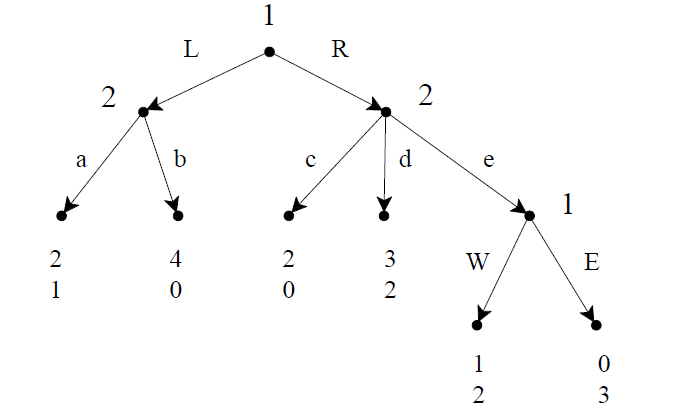
\includegraphics[width=0.45\linewidth]{Q31}
	
\end{figure}

%=========================%
%- Question 32


\item Solve the following game using Backward Induction. Express the game as a matrix game.

\begin{figure}[h!]
	\centering
	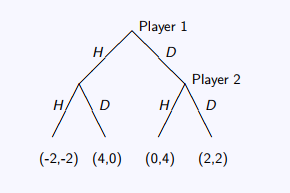
\includegraphics[width=0.4\linewidth]{Q32}
	
\end{figure}

%=========================%
%- Question 33

\item Consider the following game. Player 1 moves first and can take action A or B.
Player 2 observes the action of Player 1 and independently of the action of Player 1 can
take action A or B. Once the players have chosen their actions a die is thrown. If the
result of the die roll an odd number the payoffs obtained by the players are given by


\begin{center}
	\begin{tabular}{|c|c|c|} \hline 
		& A & B \\ \hline
		A & (2,1)& (1,3) \\ \hline
		B & (0,4) & (3,0) \\ \hline
	\end{tabular}
\end{center}
If the result of the die roll an even number the payoffs obtained by the players are given
by
\begin{center}
	\begin{tabular}{|c|c|c|} \hline 
		& A & B \\ \hline
		A & (0,8) & (6,0) \\ \hline
		B & (5,2) & (2,6) \\ \hline
	\end{tabular}
\end{center}

\begin{enumerate}[(a)]
	\item  Draw the tree depicting the extensive form of the game.
	\item Solve the component games using backward induction.
	\item  Give the matrix form of the game.
\end{enumerate}

%=========================%
%- Question 34

\item Find the Nash equilibria of the following strategic game.

\begin{center}
	\begin{tabular}{|c|c|c|} \hline 
		& L & R \\ \hline
		T & (2,2) & (0,0) \\ \hline
		B & (0,0) & (1,1) \\ \hline
	\end{tabular}
\end{center}

%=========================%
%-----------------%
%- Schaum
\item \textbf{Construct a payoff matrix far the following game.}\\

\begin{itemize}
	\item Each of two supermarket chains proposes to 
	build a store in a rural region that is served by three towns. The distances between towns are 
	shown in the figure below.\begin{figure}[h!]
		\centering
		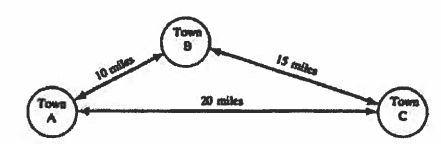
\includegraphics[width=0.45\linewidth]{Q35}
	\end{figure}
	
	\item Approximately 43 percent of the. regiions population live near town A, 33 
	percent live near town B. and 70 percent live near town C. 
	\item Because Chain 1 is larger and has 
	developed a better reputation than chain 2. chain 1 will control a majority of the business 
	whenever their situations are comparable. 
	\item 
	Both chains are aware of the other's interest in the region and both have completed marketing surveys that give identical projections.
	\item  If 
	both chains locate in the same town or equidistant from a town, chain 1 will control 65 percent of the business in that town. 
	\item
	If chain I 1 closer to a town than chain 2. chain I will control 90 mem of that towns business. 
	\item If chain 1 is farther from a town 
	than chain 2, it will still draw 40 percent of that town's business, The remaining business under all circumstances will go to chain 2. 
	\item Furthermore, both chains know that it is the policy of chain I not to locate in towns that are too small, and town C falls into this category. 
	
\end{itemize}
%-----------------%
%- Schaum
\item \textbf{Construct a payoff matrix far the following game.}\\

A barrel contains equal number of red and green marbles, Player I randomly selects one marble and inspects it (or color without showing it to player II). 

\begin{itemize}
	\item \textbf{\textit{Player I}}
	\begin{itemize}
		\item If the marble is red, player I says, "I have a red marble," and demands $\$1$ from player II.
		\item If the marble is green, either player I says, "The marble is green," and pays player II.
		\item Alternatively player I can bluff by saying, "The marble is red," and demands demands $\$1$ from player II. 
	\end{itemize}
	\item \textbf{\textit{Player II}}
	\begin{itemize}
		\item Whenever player I demands \$1, player II either can pay or can challenge player I's claim that the selected marble is red. 
		\item Once challenged, player I must show the marble to player II. 
		\item If it is indeed red. player II pays player I \$2.
		\item if it is not red, player I pays player 11 \$2. 
	\end{itemize}
	\item \textit{Use a game tree to help solve this problem.}
	\item \textit{(Hawk-Dove Game)}
\end{itemize}


%-----------------%
%% Question 37
\item \textbf{\textit{MS4315 Spring 2012 Q5  (MB / JK)}}

\begin{enumerate}[(a)]
	\item Define what is meant by a minimax strategy in a 2-player game. 
	\item For the following matrix game
	
	
	\begin{center}
		\begin{tabular}{|c|c|c|} \hline 
			& A & B \\ \hline
			A & (5,3) & (4,4) \\ \hline
			B & (2,6) & (4,4) \\ \hline
			
		\end{tabular}
	\end{center}
	Find the minimax strategies and payoffs for each player. If both players
	play their minimax strategies, what is the value of the game ? 
	\item In the context of a 2-person game, define what a Nash equilibrium is. 
	\item Does the game of part (b) have Nash equilibria ? Justify your answer.
\end{enumerate}	
%-----------------%
%% Question 38
\item \textbf{\textit{MS4315 Autumn 2014 Q5  (MB / JK)}}
\begin{enumerate}[(a)]
	\item In the context of a 2-person game, define what a Nash equilibrium is. 
	\item What is a pure strategy ? What is a mixed strategy ? 
	\item For strategies define strict dominance and weak dominance. 
	\item By removing all strategies which are dominated by strict pure or mixed
	strategies, derive the reduced version of the following 2-player matrix
	game:
	\begin{center}
		\begin{tabular}{|c|c|c|c|} \hline 
			& D & E & F \\ \hline
			A & (3,5) & (5,1) &  (1,2) \\ \hline
			B & (1,1) & (6,9) & (6,4) \\ \hline
			C & (2,6) & (4,7) & (0,8) \\ \hline
		\end{tabular}
	\end{center}
	\item  Derive the Nash equilibria and values of this game. 
\end{enumerate}
%-----------------%
%% Question 39
\item \textbf{\textit{MS4315 Autumn 2014 Q5  (MB / JK)}}

\begin{enumerate}[(a)]
	\item In the context of a 2-person game, define what a Nash equilibrium is. 
	\item What is a pure strategy ? What is a mixed strategy ? 
	\item For strategies define strict dominance and weak dominance. 
	\item By removing all strategies which are dominated by strict pure or mixed
	strategies, derive the reduced version of the following 2-player matrix
	game:
	\begin{center}
		\begin{tabular}{|c|c|c|c|} \hline 
			& D & E & F \\ \hline
			A & (4,-2)& (3,0) & (-3,-1) \\ \hline
			B & (-1,1)& (2,2) & (2,3) \\ \hline
			C & (2,1) & (-1,-1) & (0,4) \\ \hline
		\end{tabular}
	\end{center}
	\item  Derive the Nash equilibria and values of this game. 8
\end{enumerate}

%-----------------%
%% Question 40
\item \textbf{\textit{MS4315 Autumn 2015 Q5  (MB / JK)}}

%Solution is Ready
\begin{enumerate}[(a)]
	\item In terms of a strategic (matrix) game, what is a dominated strategy?
	Describe the technique of iterated elimination of dominated strategies.
	What is the technique used for ? 
	\item By removing all strategies which are dominated by strict pure or mixed
	strategies, derive the reduced version of the following 2-player zerosum
	matrix game:
	\begin{center}
		\begin{tabular}{|c|c|c|c|} \hline 
			& D & E & F \\ \hline
			A & (5,-5)& (1,-1) & (2,-2) \\ \hline
			B & (1,-1)& (0,0) & (3,-3) \\ \hline
			C & (2,-2)& (3,-3)&  (6,-6) \\ \hline
		\end{tabular}
	\end{center}
	\item In terms of a 2-player zero-sum game, what is a minimax strategy? 
	\item Derive the minimax strategies and value of the above game. 
\end{enumerate}

%-----------------%
\item \textbf{Monopoly - Introduction to Duopolies}\\% Bonanno
Let the inverse demand function and the cost function be given by
$P = 50 − 2Q$ and $C = 10 + 2q$
respectively, where Q is total industry output and q is the firm’s output. 
Cosnider the case of a monopoly ($Q=q$). Determine the optimal output level, market price, and profit for the firm.
%-----------------%
\item \textbf{Cournot Equilibrium - Introduction to Duopolies}\\% Bonanno


Determine the Cournot-Nash Equilibrium of the following Duopoly Model.

\begin{itemize}
	
	\item
	
	\item
	
\end{itemize}

%-----------------%
\item Cournot 2


Determine the Cournot-Nash Equilibrium of the following Duopoly Model.

\begin{itemize}
	
	\item
	
	\item
	
\end{itemize}
%-----------------%
\item Cournot 3

Determine the Cournot-Nash Equilibrium of the following Duopoly Model.

\begin{itemize}
	
	\item
	
	\item
	
\end{itemize}

%-----------------%
\item \textbf{Bertrand Duopoly 1 (Identical Goods)}

%- Sporting Clay

Determine the Bertrand Equilibrium of the following Duopoly Model.

\begin{itemize}
	
	\item
	
	\item
	
\end{itemize}
%-----------------%
\item \textbf{Bertrand Duopoly 2 (Different Goods)}

%- Sporting Clay

Determine the Bertrand Equilibrium of the following Duopoly Model.

\begin{itemize}
	
	\item
	
	\item
	
\end{itemize}
%-----------------%
\item \textbf{Stackleberg Quantity Leadership Problem}
%- Lady


Determine the Stackleberg Equilibrium of the following Duopoly Model.

\begin{itemize}
	
	\item
	
	\item
	
\end{itemize}

%-----------------%
\item \textbf{Stackleberg : 2 Firm with Identical Goods}
%- Sporting Clay
Determine the Stackleberg Equilibrium of the following Duopoly Model.

\begin{itemize}
	
	\item
	
	\item
	
\end{itemize}
%=============================%
\item \textbf{Cartel Question}\\
Consider an industry with two firms. Firms are identical and produce an
homogenous product. Firms have to select outputs (capacity) in order to maximize
profits. Each firm knows its own total cost of production, the total cost of production of
the competitor and the industry demand.
\\
The following data are known by both firms and describe the industry
situation:
\begin{itemize}
\item P = 140 - (Q1+Q2) \textit{(industry demand)}
\item TC1 = 20Q1 \textit{(total cost of firm 1),}
\item TC2 = 20Q2 \textit{(total cost of firm 2).}
\end{itemize}
Suppose that both firms agree to form a cartel. The goal of the cartel is to set the
industry output at a level that maximizes industry profits. A rule governing the cartel
behavior specifies how the industry output and profits must be shared among the cartel
members.
\item \textbf{MS4315 Autumn 2013 Combined Duopoly Question}\\
Consider the asymmetric duopoly game: Firm i, i = 1, 2 produces xi
items
at a cost of
\[C(x_i) = \frac{1}{i}x_i + 20.\]
The items sell at a price of
\[p(x1, x2) = 5 − \frac{x_1+x_2}{500}\]
each.
\begin{enumerate}[(a)]
	\item Find the equilibrium of the game if it is played as a Cournot game,
	and prove that it is a Nash equilibrium. 
	\item Find the equilibrium if it played as a Stackelberg game with Firm 1 as
	leader. 
	\item Contrast and comment on the two solutions. 
\end{enumerate}

%-----------------%

\item \textbf{(\textit{From a Previous Exam Paper})} \\ In a game show, contestants M\'{a}ire and S\'{e}amus start the last round with \euro{500} and \euro{400} respectively. Each must decide to pass or play. If a player passes, they keep their money but if they opt to play they win or lose \euro{200} each with probability 1/2. These outcomes are independent of each other. The player with the most money at the end of the round gets a bonus of \euro{300}.

\begin{enumerate}
	\item[(a)] If M\'{a}ire goes first and S\'{e}amus sees her move, draw the game tree. 
	\item[(b)] Show that the strategic form of the game is
	
	\begin{center}
		
		\begin{tabular}{|c|c|c|}
			\hline
			& Pass         &Play       \\
			\hline
			Pass & (8,4) &$\left(\frac{13}{2}, \frac{11}{2}\right)$  \\
			\hline
			Play & $\left(\frac{13}{2}, \frac{11}{2}\right)$& $\left(\frac{29}{4}, \frac{19}{4}\right)$ \\
			\hline
		\end{tabular}
	\end{center}
	where payoffs are expected values in 00's. 
	
	\item[(c)] Solve the game using Backward Induction.
\end{enumerate}
%================%
%- Question 52

\item \textbf{(\textit{From a Previous Exam Paper})} \\ In a game show, contestants S\'{i}le and S\'{e}an start the last round with \euro{500} and \euro{400} respectively. Each must decide to pass or play. If a player passes, they keep their money but if they opt to play they win or lose \euro{200} each with probability 1/2. These outcomes are independent of each other. The player with the most money at the end of the round gets a bonus of \euro{200}.

\begin{enumerate}
	\item[(a)] Suppose S\'{i}le goes first, with S\'{e}an then taking his turn, after seeing her move. Draw the game tree. 
	\item[(b)] Show that the strategic form of the game is
	
	\begin{center}
		
		\begin{tabular}{|c|c|c|}
			\hline
			& Pass         &Play       \\
			\hline
			Pass & (7,4) &$\left(6, 5 \right)$  \\
			\hline
			Play & $\left(6, 5 \right)$ & $\left(\frac{9}{2}, 5\right)$ \\
			\hline
		\end{tabular}
	\end{center}
	where payoffs are expected values in 00's. 
	
	\item[(c)] Solve the game using Backward Induction.
\end{enumerate}


\item \textbf{Binary Classification Question (Decision Theory)}\\
Consider the following confusion matrix.(The total number of experiments is 10,000)
\begin{center}
	\begin{tabular}{|c|c|c|}
		\hline 
		& 	Predict Negative & Predict Positive \\ 
		\hline 
		Observed Negative	& 9700 & 80 \\ 
		\hline 
		Observed Positive	& 100  &  120 \\ 
		\hline 
	\end{tabular} 
\end{center}
Compute the following measurements
\begin{multicols}{2}
	\begin{enumerate}
		\item Accuracy \item Recall \item Precision \item The F-measure
	\end{enumerate}
\end{multicols}
\item Explain the class imbalance problem in binary 
classification procedures. Explain how this would advserely affect some
performance measures for binary classification procedures.
\item %  Binary Classification (4 Marks)
For following binary classification outcome table (i.e. confusion matrices), calculate the following appraisal metrics.

\begin{multicols}{2}
	\begin{enumerate}[(a)]
		\item Accuracy;
		\item Recall
		\item Precision;
		\item F-measure.
	\end{enumerate}
\end{multicols}
\noindent \textbf{Confusion Matrix 1} \smallskip
\begin{center}
	
	\begin{tabular}{|c||c|c|}
		\hline 
		& Predict Negative & Predict Positive \\ \hline  \hline 
		Observed Negative & 9560 &  100 \\ \hline 
		Observed Positive & 270 & 70 \\ \hline 
	\end{tabular} 
\end{center}
\noindent \textbf{Confusion Matrix 2}
\begin{center}
	\begin{tabular}{|c||c|c|}
		\hline 
		& Predict Negative & Predict Positive \\ \hline  \hline 
		Observed Negative & 9500 &  320 \\ \hline 
		Observed Positive & 20 & 160 \\ \hline 
	\end{tabular} 
\end{center}
\item Decision Theory (Bayes Test)
\item Binary Classification
\item \textbf{Monopoly Question (MS4315 Mark Burke)}\\
The costs incurred by a firm in a production period are
$c = 100 + 2x$
where x is the number of items produced in that period. The items each sell
at a price of
\[P(x) = 10 - \frac{x}{50}. \]
Find the level of production that maximises the firm’s profits
when the firm has a monopoly.
 \item
 \begin{enumerate}[(a)]
 	\item Big O-notation is used to classify algorithms according to their relative complexity. Compare the complexity of algorithms of order $\mathrm{O}(\log n)$, $\mathrm{O}(n)$, $\mathrm{O}(n\log n)$, $\mathrm{O}(2^n)$and $\mathrm{O}(n!)$. Illustrate your answer with a sketch. 
 	\item Classify the Binary Search Tree algorithm using Big $\mathrm{O}$-notation. Justify your answer. 
 	\item Compare and contract Big O-Notation, Big Omega Notation and Big Theta Notation. 
 	
 	\item What is meant by Combinatorial Explosion? Why is it relevant for Binary Integer Problems? 
 	
 \end{enumerate}

%===================================%
% Question 60
\item \textbf{Algorithm Definition Questions}
\begin{multicols}{2}
	\begin{itemize}

		\item Knapsack Problem
		\item Provide illustrations / Examples
	\end{itemize}
\end{multicols}
 	



\end{enumerate}


\end{document}